% MORPH — Context Coverage at Scale.
% Two parallel coverage lanes over ONE shared causal axis [0,i] (NOT a nested hierarchy):
%   - Even layers: CSA branch  -> sparse top-128 of S/4 fine (4-tok) blocks, anywhere in [0,i].
%   - Odd  layers: HCA branch  -> dense over all S/128 coarse (128-tok) blocks.
%   - Both layers also run the local sliding window (last w=128 tokens, per-token).
% CSA and HCA ALTERNATE by layer parity (never simultaneous). All attention causal [0,i].
%
% Nesting fact (shown in the inset): CSA & HCA block boundaries COINCIDE
%   (1 HCA block = 32 CSA blocks, since 128 = 32*4, both tile from token 0), BUT the two are
%   pooled INDEPENDENTLY (separate compressors, different layers) — neither is built from the other.
%
% Verified vs morph/model/attention.py + configs/base.yaml:
%   csa_compress_ratio=4, hca_compress_ratio=128, top_k=128, window_size=128.
%   CSA: _CCACSAAttention (compressor two_stream=True) + LightningIndexer + topk (top-128 anywhere).
%   HCA: _CCAHCAAttention (compressor two_stream=False), dense over all blocks.
%   Window: _CCABase._window_attn, always on, both branches.  n_blocks = S // m (computed live).
%   Illustrative S=1M (1,048,576); block sizes symbolic in S (n_blk = S/m).
% Compile: pdflatex morph_context_coverage.tex

\documentclass[border=14pt]{standalone}
\usepackage[T1]{fontenc}
\usepackage{amsmath,amssymb}
\usepackage{tikz}
\usetikzlibrary{arrows.meta, calc, decorations.pathreplacing, positioning}

% ── Palette (Paul Tol, colorblind-safe — matches the figure family) ───────────
\definecolor{cbBlue}{HTML}{4477AA}
\definecolor{cbOrange}{HTML}{EE7733}
\definecolor{cbPurple}{HTML}{AA3377}
\definecolor{cbTeal}{HTML}{228833}
\definecolor{cbGray}{HTML}{777777}
\definecolor{fOrange}{HTML}{FDE8D0}
\definecolor{fPurple}{HTML}{EEDCEE}
\definecolor{fTeal}{HTML}{D6EFDD}
\definecolor{winLine}{HTML}{2A5599}   % local window — distinct blue (clearly shared by both branches)
\definecolor{winFill}{HTML}{BBD0EF}
\definecolor{bdr}{HTML}{555555}

\tikzset{
  capt/.style={font=\footnotesize\sffamily, align=center},
  sub/.style={font=\scriptsize\sffamily},
  tny/.style={font=\tiny\sffamily, text=cbGray},
}

\begin{document}
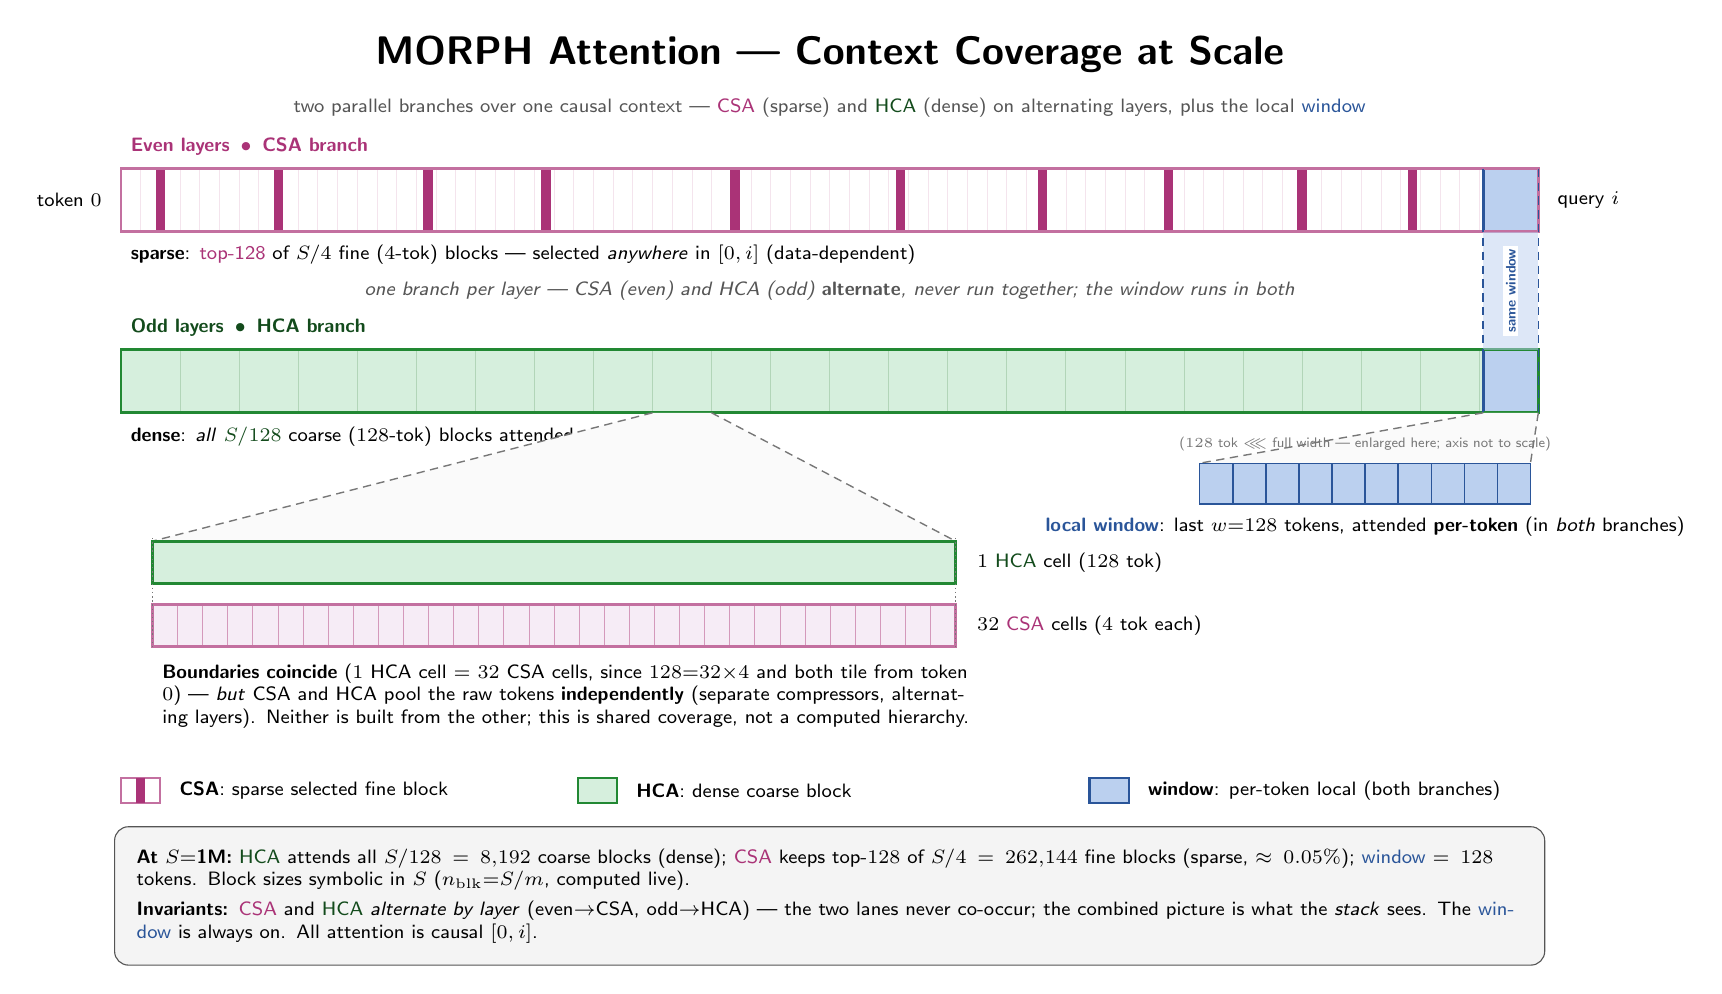
\begin{tikzpicture}

\def\xL{-9}  \def\xR{9}
\def\hh{0.40}            % lane half-height
\def\yc{5.55}           % CSA lane centre (even layers)
\def\yh{3.25}           % HCA lane centre (odd layers)
\def\wL{8.30}           % window slab left edge (right end of every lane)

% =====================================================================
% LANE 1 — Even layers: CSA (sparse) + window
% =====================================================================
\fill[white] (\xL,\yc-\hh) rectangle (\xR,\yc+\hh);
% faint dense fine grid (suggests the S/4 fine blocks)
\foreach \i in {1,...,71}{ \pgfmathsetmacro\x{\xL + \i*0.25}
  \draw[cbPurple!13, line width=0.25pt] (\x,\yc-\hh) -- (\x,\yc+\hh); }
% the few SELECTED fine blocks — scattered ANYWHERE, mostly empty => visually sparse
\foreach \x in {-8.5,-7.0,-5.1,-3.6,-1.2,0.9,2.7,4.3,6.0,7.4,8.6}{
  \fill[cbPurple] (\x-0.06,\yc-\hh) rectangle (\x+0.06,\yc+\hh); }
% window slab (right end)
\fill[winFill] (\wL,\yc-\hh) rectangle (\xR,\yc+\hh);
\draw[winLine, line width=1.1pt] (\wL,\yc-\hh) rectangle (\xR,\yc+\hh);
\draw[cbPurple!70, line width=1pt] (\xL,\yc-\hh) rectangle (\xR,\yc+\hh);
% labels
\node[sub, anchor=south west, text=cbPurple] at (\xL,\yc+\hh+0.05)
  {\textbf{Even layers \,$\bullet$\, CSA branch}};
\node[sub, anchor=north west] at (\xL,\yc-\hh-0.05)
  {\textbf{sparse}: \textcolor{cbPurple}{top-128} of $S/4$ fine ($4$-tok) blocks --- selected \emph{anywhere} in $[0,i]$ (data-dependent)};
\node[sub, anchor=east] at (\xL-0.12,\yc) {token $0$};
\node[sub, anchor=west] at (\xR+0.12,\yc) {query $i$};

% alternation note between lanes
\node[font=\scriptsize\sffamily\itshape, text=bdr] at (0,0.5*\yc+0.5*\yh)
  {one branch per layer --- CSA (even) and HCA (odd) \textbf{alternate}, never run together; the window runs in both};

% =====================================================================
% LANE 2 — Odd layers: HCA (dense) + window
% =====================================================================
\fill[fTeal] (\xL,\yh-\hh) rectangle (\xR,\yh+\hh);
\foreach \i in {1,...,23}{ \pgfmathsetmacro\x{\xL + \i*0.75}
  \draw[cbTeal!35, line width=0.3pt] (\x,\yh-\hh) -- (\x,\yh+\hh); }
\fill[winFill] (\wL,\yh-\hh) rectangle (\xR,\yh+\hh);
\draw[winLine, line width=1.1pt] (\wL,\yh-\hh) rectangle (\xR,\yh+\hh);
\draw[cbTeal, line width=1pt] (\xL,\yh-\hh) rectangle (\xR,\yh+\hh);
\node[sub, anchor=south west, text=cbTeal!55!black] at (\xL,\yh+\hh+0.05)
  {\textbf{Odd layers \,$\bullet$\, HCA branch}};
\node[sub, anchor=north west] at (\xL,\yh-\hh-0.05)
  {\textbf{dense}: \emph{all} \textcolor{cbTeal!55!black}{$S/128$} coarse ($128$-tok) blocks attended};

% shared-window column: the SAME window is attended by both branches
\fill[winFill, opacity=0.5] (\wL,\yh+\hh) rectangle (\xR,\yc-\hh);
\draw[winLine, densely dashed, line width=0.6pt] (\wL,\yc+\hh) -- (\wL,\yh-\hh);
\draw[winLine, densely dashed, line width=0.6pt] (\xR,\yc+\hh) -- (\xR,\yh-\hh);
\node[font=\tiny\sffamily\bfseries, text=winLine, fill=white, inner sep=1pt, rotate=90]
  at (0.5*\wL+0.5*\xR, 0.5*\yc+0.5*\yh) {same window};

% =====================================================================
% WINDOW magnifier (right) — make the local window obvious + handle scale
% =====================================================================
\def\mxa{4.7}\def\mxb{8.9}\def\myc{1.95}\def\mhh{0.26}
\fill[cbGray!4] (\wL,\yh-\hh) -- (\xR,\yh-\hh) -- (\mxb,\myc+\mhh) -- (\mxa,\myc+\mhh) -- cycle;
\draw[densely dashed, cbGray, line width=0.5pt] (\wL,\yh-\hh) -- (\mxa,\myc+\mhh);
\draw[densely dashed, cbGray, line width=0.5pt] (\xR,\yh-\hh) -- (\mxb,\myc+\mhh);
\foreach \j in {0,...,9}{ \pgfmathsetmacro\xa{\mxa + \j*((\mxb-\mxa)/10)}
  \pgfmathsetmacro\xb{\xa + (\mxb-\mxa)/10}
  \fill[winFill] (\xa,\myc-\mhh) rectangle (\xb,\myc+\mhh);
  \draw[winLine, line width=0.5pt] (\xa,\myc-\mhh) rectangle (\xb,\myc+\mhh); }
\node[sub, anchor=north, align=center] at (0.5*\mxa+0.5*\mxb,\myc-\mhh-0.04)
  {\textbf{\textcolor{winLine}{local window}}: last $w{=}128$ tokens, attended \textbf{per-token} (in \emph{both} branches)};
\node[tny, anchor=south] at (0.5*\mxa+0.5*\mxb,\myc+\mhh+0.03)
  {($128$ tok $\lll$ full width --- enlarged here; axis not to scale)};

% =====================================================================
% NESTING inset (left) — one HCA cell == 32 CSA cells, boundary-aligned, independent
% =====================================================================
% source: one coarse HCA cell on lane 2 (x in [-2.25,-1.50])
\def\sca{-2.25}\def\scb{-1.50}
\def\ixa{-8.6}\def\ixb{1.6}
\def\iyT{0.95}\def\iyB{0.15}\def\ihh{0.27}
\fill[cbGray!4] (\sca,\yh-\hh) -- (\scb,\yh-\hh) -- (\ixb,\iyT+\ihh) -- (\ixa,\iyT+\ihh) -- cycle;
\draw[densely dashed, cbGray, line width=0.5pt] (\sca,\yh-\hh) -- (\ixa,\iyT+\ihh);
\draw[densely dashed, cbGray, line width=0.5pt] (\scb,\yh-\hh) -- (\ixb,\iyT+\ihh);
% top sub-row: ONE HCA cell
\fill[fTeal] (\ixa,\iyT-\ihh) rectangle (\ixb,\iyT+\ihh);
\draw[cbTeal, line width=1pt] (\ixa,\iyT-\ihh) rectangle (\ixb,\iyT+\ihh);
\node[sub, anchor=west] at (\ixb+0.15,\iyT) {$1$ \textcolor{cbTeal!55!black}{HCA} cell ($128$ tok)};
% bottom sub-row: 32 CSA cells
\foreach \j in {0,...,31}{ \pgfmathsetmacro\xa{\ixa + \j*((\ixb-\ixa)/32)}
  \pgfmathsetmacro\xb{\xa + (\ixb-\ixa)/32}
  \fill[fPurple!55] (\xa,\iyB-\ihh) rectangle (\xb,\iyB+\ihh);
  \draw[cbPurple!50, line width=0.3pt] (\xa,\iyB-\ihh) rectangle (\xb,\iyB+\ihh); }
\draw[cbPurple!70, line width=1pt] (\ixa,\iyB-\ihh) rectangle (\ixb,\iyB+\ihh);
\node[sub, anchor=west] at (\ixb+0.15,\iyB) {$32$ \textcolor{cbPurple}{CSA} cells ($4$ tok each)};
% aligned-boundary guides at the shared edges
\draw[cbGray, densely dotted, line width=0.5pt] (\ixa,\iyT+\ihh+0.04) -- (\ixa,\iyB-\ihh-0.04);
\draw[cbGray, densely dotted, line width=0.5pt] (\ixb,\iyT+\ihh+0.04) -- (\ixb,\iyB-\ihh-0.04);
\node[sub, anchor=north west, align=left, text width=10.3cm] at (\ixa,\iyB-\ihh-0.10)
  {\textbf{Boundaries coincide} ($1$ HCA cell $=32$ CSA cells, since $128{=}32{\times}4$ and both tile from token $0$) --- \emph{but} CSA and HCA pool the raw tokens \textbf{independently} (separate compressors, alternating layers). Neither is built from the other; this is shared coverage, not a computed hierarchy.};

% =====================================================================
% Legend + invariants
% =====================================================================
\def\ly{-1.95}
\fill[white, draw=cbPurple!70, line width=0.8pt] (\xL,\ly-0.16) rectangle (\xL+0.5,\ly+0.16);
\fill[cbPurple] (\xL+0.19,\ly-0.16) rectangle (\xL+0.31,\ly+0.16);
\node[sub, anchor=west] at (\xL+0.62,\ly) {\textbf{CSA}: sparse selected fine block};
\fill[fTeal, draw=cbTeal, line width=0.8pt] (-3.2,\ly-0.16) rectangle (-2.7,\ly+0.16);
\node[sub, anchor=west] at (-2.58,\ly) {\textbf{HCA}: dense coarse block};
\fill[winFill, draw=winLine, line width=0.8pt] (3.3,\ly-0.16) rectangle (3.8,\ly+0.16);
\node[sub, anchor=west] at (3.92,\ly) {\textbf{window}: per-token local (both branches)};

\node[draw=bdr, rounded corners=5pt, fill=cbGray!8, inner sep=8pt, anchor=north,
      align=left, font=\scriptsize\sffamily, text width=17.6cm] at (0,\ly-0.45) {%
  \textbf{At $S{=}$1M:} \textcolor{cbTeal!55!black}{HCA} attends all $S/128 = 8{,}192$ coarse blocks (dense); \textcolor{cbPurple}{CSA} keeps top-$128$ of $S/4 = 262{,}144$ fine blocks (sparse, $\approx0.05\%$); \textcolor{winLine}{window} $=128$ tokens. Block sizes symbolic in $S$ ($n_\mathrm{blk}{=}S/m$, computed live).\\[3pt]
  \textbf{Invariants:} \textcolor{cbPurple}{CSA} and \textcolor{cbTeal!55!black}{HCA} \emph{alternate by layer} (even$\to$CSA, odd$\to$HCA) --- the two lanes never co-occur; the combined picture is what the \emph{stack} sees. The \textcolor{winLine}{window} is always on. All attention is causal $[0,i]$.};

% =====================================================================
% Title
% =====================================================================
\node[font=\Large\sffamily\bfseries, anchor=south] (ttl) at (0,7.05)
  {MORPH Attention --- Context Coverage at Scale};
\node[sub, text=bdr, anchor=north, below=0.08cm of ttl, text width=17cm, align=center]
  {two parallel branches over one causal context --- \textcolor{cbPurple}{CSA} (sparse) and \textcolor{cbTeal!55!black}{HCA} (dense) on alternating layers, plus the local \textcolor{winLine}{window}};

\end{tikzpicture}
\end{document}
